% this file is called up by thesis.tex
% content in this file will be fed into the main document

%------------------------------------------------------------------------- 

\chapter{Introducción y marco teórico}
\label{cha:Gen_intro}

\graphicspath{{Figures/ch2_img/}{../Figures/ch2_img/}}

\section{Marco Teórico y Estado del arte}
\label{sec:marco_teorico}

Los haces con OAM distinto de cero inicialmente fueron generados en el
laboratorio por medio de técnicas analógicas entre las que se destacan
el uso de conversores modales \cite{Alekseev1998}, placas de fase espiral grabadas en sustratos
transparentes \cite{Jun2009}, y hologramas de fase impresos en acetato
\cite{Carpentier2008} . La conversión modal utiliza sucesiones de
lentes astigmáticas para convertir los modos Hermite Gauss en modos
Laguerre Gauss, y fue la primera forma en la cual se produjeron VO en
el laboratorio. A diferencia de la conversión modal, - que requiere un
montaje experimental muy sensible -  las técnicas que utilizan máscaras
de fase se caracterizan por necesitar sólo un elemento óptico que
permite modificar punto a punto la fase de un haz que originalmente
carecía de momento angular, para convertirlo en un haz con vorticidad
óptica. El uso de placas físicas grabadas con un patrón espiral
tiene la ventaja de generar haces LG con sólo ubicarlas en
el camino óptico del haz, y tiene la desventaja de que una vez
fabricadas no se pueden modificar. 
En situaciones donde es requerido generar haces del tipo LG con la suficiente
flexibilidad como para corregir aberraciones ópticas, se
necesita de dispositivos digitales con propiedades similares a los
dispositivos analógicos mencionados anteriormente. Estos dispositivos
se conocen como moduladores espaciales de luz o SLM por sus siglas en
inglés. En este proyecto se pretende generar VO y caracterizar su
frente de onda utilizando un tipo de SLM's que modifican la fase de la
luz cuando ésta pasa a través de ellos. 

\subsection{Moduladores Espaciales de Luz}

Como su nombre lo indica, los moduladores espaciales de luz sirven
para modular punto a punto las propiedades de la luz sobre un
plano. Ya sea solamente su amplitud como en los dispositivos de
visualización de cristal líquido (pantallas LCD), o su fase como en
los dispositivos que se ilustran en la figura \ref{fig:LCDSLM}.
\begin{figure}[h!]
\centering
    \includegraphics[width=0.5\textwidth]{LCDSLM.png}
\caption{Moduladores espaciales PLUTO y LC2012 de reflexión y
  transmisión marca Holoeye basados en la tecnología de cristal
  líquido. Por ser hecho a partir de un LCD comercial el modulador de
  la derecha es ensamblado a una cuarta parte del costo del izquierdo.}
\label{fig:LCDSLM}
\end{figure}

Si diferenciamos los SLM por el tipo de tecnología, estos pueden ser
agrupados en dos categorías: basados en cristales líquidos, o en
arreglos de micro espejos (figura \ref{fig:MEMSLM}), mejor 
conocidos en la industria de la proyección como DLP (de Digital Light
Processing).  
\subsubsection{Moduladores basados en micro espejos}
En su mayoría, los moduladores comerciales basados en arreglos de micro
espejos funcionan con micro mecanismos que inclinan la superficie
reflectiva de tal forma que se modifique la cantidad de luz que un
observador ve desde una perspectiva dada, es decir que modulan
intensidad. Sin embargo, con el interés de modular fase además de
intensidad se han desarrollado nuevos micro mecanismos que
permiten desplazar verticalmente el espejo sin modificar su
inclinación introduciendo así un cambio en la longitud del camino
óptico y por ende la fase tal y como se presenta en \cite{Wu2010,
  Liesener2006}. Dado que es una tecnología incipiente y ha tenido
menor tiempo en el mercado que los cristales líquidos, estos sistemas
y en particular los de tipo pistón, siguen teniendo precios elevados y
aún están lejos de ser utilizados en muchos laboratorios.

\begin{figure}[h!]
\centering
    \includegraphics[width=0.5\textwidth]{MEMSLM.png}
\caption{Modulador espacial basado en arreglos de micro espejos marca Texas Instruments.}
\label{fig:MEMSLM}
\end{figure}

\subsubsection{Moduladores de cristal líquido}
Los SLM basados en Cristales Líquidos (CL) aprovechan las propiedades
físicas de ciertos polímeros que dada su forma alargada y propiedades
electrónicas polares, cambian su orientación ante la presencia de
campos eléctricos.  Esta sensibilidad a los campos eléctricos, en
conjunto con sus propiedades ópticas anisotrópicas permitió que desde
los años 70s se implementaran CL para generar imágenes en pantallas de
dispositivos como relojes, calculadoras y luego televisores y
proyectores. Fue más adelante cuando estudios más especializados de las
propiedades de los cristales líquidos como los realizados por Yariv y Yeh
en \cite{Yeh1999,Yariv2002}, y experimentos como los de Konforti et
al. \cite{Konforti1988} demostraron que los LCD pueden ser usados como
moduladores de solo fase. 
Aunque la aplicación de cristales líquidos para modulación de fase es
relativamente reciente, el estudio de sus propiedades físicas no lo es
y desde los años 60’s la investigación ha sido respaldada por grandes
empresas interesadas en desarrollar productos tecnológicos de
generación y procesamiento de imágenes como RTC, Hamamatsu, Hitachi, HP, Texas
Instruments, Sony y otros. Dado este interés por entender los CL, se
ha llegado a modelos matemáticos y  técnicas de  
caracterización robustas que permiten extraer los parámetros de un SLM para
 simular su comportamiento.
El desarrollo de estas técnicas ha permitido a investigadores 
alrededor del mundo implementar moduladores de fase a
partir de elementos LCD extraídos de dispositivos de proyección
comerciales, entre ellos se encuentran los trabajos de
\cite{Pezzaniti1993,Soutar1994,Zhang1994,Moreno1998,Davis1999,Iemmi2001,Davis2003,Moreno2003,Kim2005,Duran2006,Duran2007,Marquez2007,Liu2010,Ma2010,Ma2011,Yu2012}. Mientras
que autores como Mahmud, \cite{Mahmud2008}, Roopahsree
\cite{Roopashree2009a}, y David \cite{Dev2012}
caracterizaron un Holoeye LC2002 que es vendido comercialmente como
modulador de amplitud y fase.
Ejemplo de la práctica de reensamblar un LCD y venderlo como SLM es el
modulador marca Holoeye LC2012 que gracias a usar un LCD comercial
marca Sony es ensamblado a una cuarta parte del precio de otros
moduladores. 

Adicionalmente, cabe mencionar que los moduladores en base a CL se
dividen en dos tipos, de reflexión y de transmisión. Sin entrar en
detalle, los primeros permiten modulaciones de fase que van hasta $2\pi$
radianes, tienen mayor resolución, necesitan menos elementos de
polarización para su uso, tienen altas velocidades de operación y el
hecho de que la electrónica esté detrás del cristal (y detrás de la
superficie reflectiva) hace que se produzcan menos efectos indeseados
de difracción. Todo esto a costa de desarrollar CL y
electrónica personalizados. En cambio, los moduladores de transmisión
se desarrollan a partir de CL comerciales que fuera de polarizar la luz
retardan su fase. Esto implica un acople entre modulación de fase y 
modulación de intensidad que se traduce en menor calidad de la
modulación de fase total. Para lograr una buena
modulación se necesitan polarizadores y retardadores que generan un
estado de polarización específico a la entrada del SLM. Por otra
parte, al tener la electrónica acoplada sobre el cristal, se limita la
resolución; no todo el volumen de CL se aprovecha y se introducen
efectos indeseados de difracción. 
No obstante, los SLM de transmisión son muy económicos y algunos
autores como Davis et al. \cite{Davis2000, Davis2013} han propuesto
que se podrían usar como dispositivos para modular polarización. En
base a esto otros como Moreno et al. \cite{Moreno2004, Moreno2011} han
combinado el formalismo de Fourier con el de las matrices de Jones
para modelar el comportamiento de dispositivos ópticos de Fourier que
involucran polarización. 
En el laboratorio de metrología óptica del grupo de Óptica Aplicada se
encuentran dos moduladores de transmisión marca Holoeye modelos
LC-2002 y LC- 2012 que necesitan ser caracterizados para optimizar su
uso en aplicaciones metrológicas tales como la creación de vórtices
ópticos. 
La generación de VO se da entonces una vez se tenga apropiada la
herramienta que los produce. El resto de esta sección se enfoca en la
segunda mitad del problema, es decir, ¿Cómo caracterizar y corregir las
aberraciones ópticas de un VO?

\subsection{Aberraciones ópticas}

Los VO generados en el laboratorio están sujetos a aberraciones
ópticas que se asocian a situaciones tales como:
\begin{itemize}
\item Problemas en la alineación de componentes ópticos como
  lentes o espejos.
\item Deformaciones en las superficies de elementos como
  polarizadores, lentes, espejos, láminas retardadoras, e incluso de
  las céldas de cristal líquido en el SLM.
\item Presencia de partículas de polvo en las superficies de las
  componentes ópticas que inducen efectos indeseados de difracción. 
\end{itemize}

Adicionalmente, y siguiendo con el tema de la sección anterior, los
SLM de transmisión basados en pantallas de CL introducen otras fuentes
de aberraciones. En primera medida, las pantallas son dispositivos discretos en dos de los
sentidos de la palabra. Por un lado, son discretos espacialmente y
las señales de control son asignadas a subdivisiones del cristal de tamaño finito
conocidas como pixeles. El arreglo rectangular de todos los pixeles
genera efectos de difracción similares a los de rejillas verticales y
horizontales combinadas. Esto quiere decir que el SLM separa los
órdenes de difracción de la luz que pasa a travez de él. Asimismo, el
hecho de ser una cuadrícula discreta hace que el modulador obviamente no pueda
generar distribuciones de fase en regiones infinitamente pequeñas como sería deseado
alrededor de una singularidad óptica. Como ejemplo, en la figura
\ref{fig:discrete_mask} a) se muestra una imagen del la máscara que se
envía al SLM en la región donde resultaría una singularidad
óptica. Como se puede ver, la máscara de fase discreta resulta muy distinta a
la máscara ideal que se presentó en la figura \ref{fig:oam_intro}b), y
por lo tanto introduce deformaciones en el haz Laguerre-Gauss que
resulta a la salida del SLM.   

\begin{figure}[h!]
\centering
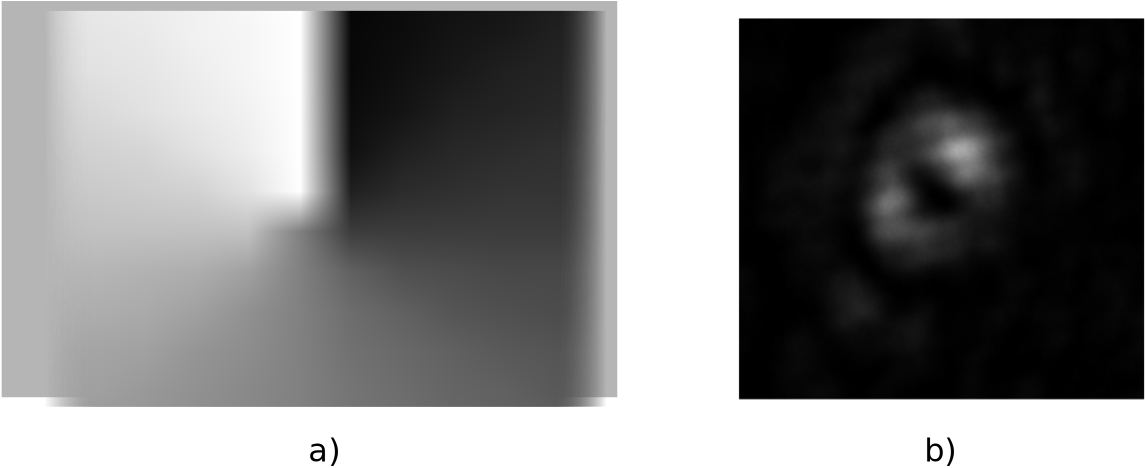
\includegraphics[ scale=.4]{discrete_mask.png}
%Las imagenes que enviamos al SLM son generadas en un
%  ordenador que de por sí es discreto, y llegan a un dispositivo
 % físico que tiene divisiones discretas, tanto espaciales como
 % electrónicas. Aún 
\caption{a) Magnificación de una mascara tipica proyectada al SLM. b) Imagen de un VO de poca calidad producido con un SLM de
transmisión modelo Holoeye LC2002.}
\label{fig:discrete_mask}
\end{figure}

Por otra parte, el SLM es discreto en la medida que sólo puede asignar
níveles de voltaje discretos (0-255 divisiónes de 5V) a cada una de
las celdas. Este fenómeno también es observable en la figura
\ref{fig:discrete_mask}a) y puede introducir efectos
indeseados. Más aún, si cómo el nuestro, el modulador no llega a una
modulación de sólo fase, o tiene una modulación que no llega a
completar el ciclo de $2\pi$ radianes. 
Todas las posibles fuentes de error mencionadas anteriormente se
combinan para generar haces Laguerre-Gauss de poca calidad como el que se muestra
en la figura \ref{fig:discrete_mask} b). 

\newpage
\pagebreak[4]
\bibliographystyleInt{unsrtnat}
\bibliographyInt{References/Int}